\chapter{Apache Spark and Spark Streaming}
\label{spark}

\section{Introduction}
\label{sp:intro}

Apache Spark~\cite{spark} is a general purpose data processing framework that supports wide range of applications from \emph{batch} processing, \emph{stream} processing, \emph{graph} processing to \emph{machine learning}, etc. In this chapter the architecture of Apache Spark and Spark Streaming -- as one of its sub projects -- will be explored and discussed. Throughout the chapter, minor examples will also be presented to further simplify the concepts. This chapter is organized as follows. Section~\ref{sp:basics} explains the basic concepts of Apache Spark. Then, section~\ref{sp:rdd} explains \emph{Resilient Distributed Datasets} (RDDs) which is the most integral component of the Apache Spark. Section~\ref{sp:dstream} explains \emph{Discretized Streams} (DStreams) as the fundamental building block for data stream processing applications. Finally, section~\ref{sp:conc} concludes this chapter.

\section{Basic Concepts}
\label{sp:basics}

Map-Reduce~\cite{Dean:2004} and its derivative projects have been widely used by \emph{data-oriented} applications to process and crunch huge datasets over last the decade. In traditional Map-Reduce environments, developers typically create \emph{acyclic} data flow graphs to process input data. However, as confirmed by \textcite{Zaharia:2010}, there are two categories of applications that are not well suited for this architecture.
\begin{itemize}
    \item \textbf{Iterative Jobs} Many machine learning applications process the same input \emph{iteratively}. In traditional model, each iteration should be defined as a separate MapReduce job. While this is feasible, but for each job, input data has to be loaded from disk which leads to serious performance issues.
    \item \textbf{Interactive Analysis} MapReduce derivative projects like Hive~\cite{hive} and Pig~\cite{pig} have been extensively used to run SQL queries on top of massive datasets. Whenever a user submits different queries over the same dataset, the ideal solution would be to load all datasets into memory once and then execute different queries on top of it. However, with traditional model of execution each query shall be defined as a separate job which reads input data from disk.
\end{itemize}
Apache spark has been designed from ground up to resolve these issues. It provides a large stack of tools to facilitate processing large datasets. Figure~\ref{fig:spark-eco} depicts tools provided by Spark.
\begin{figure}[h]
    \centering
    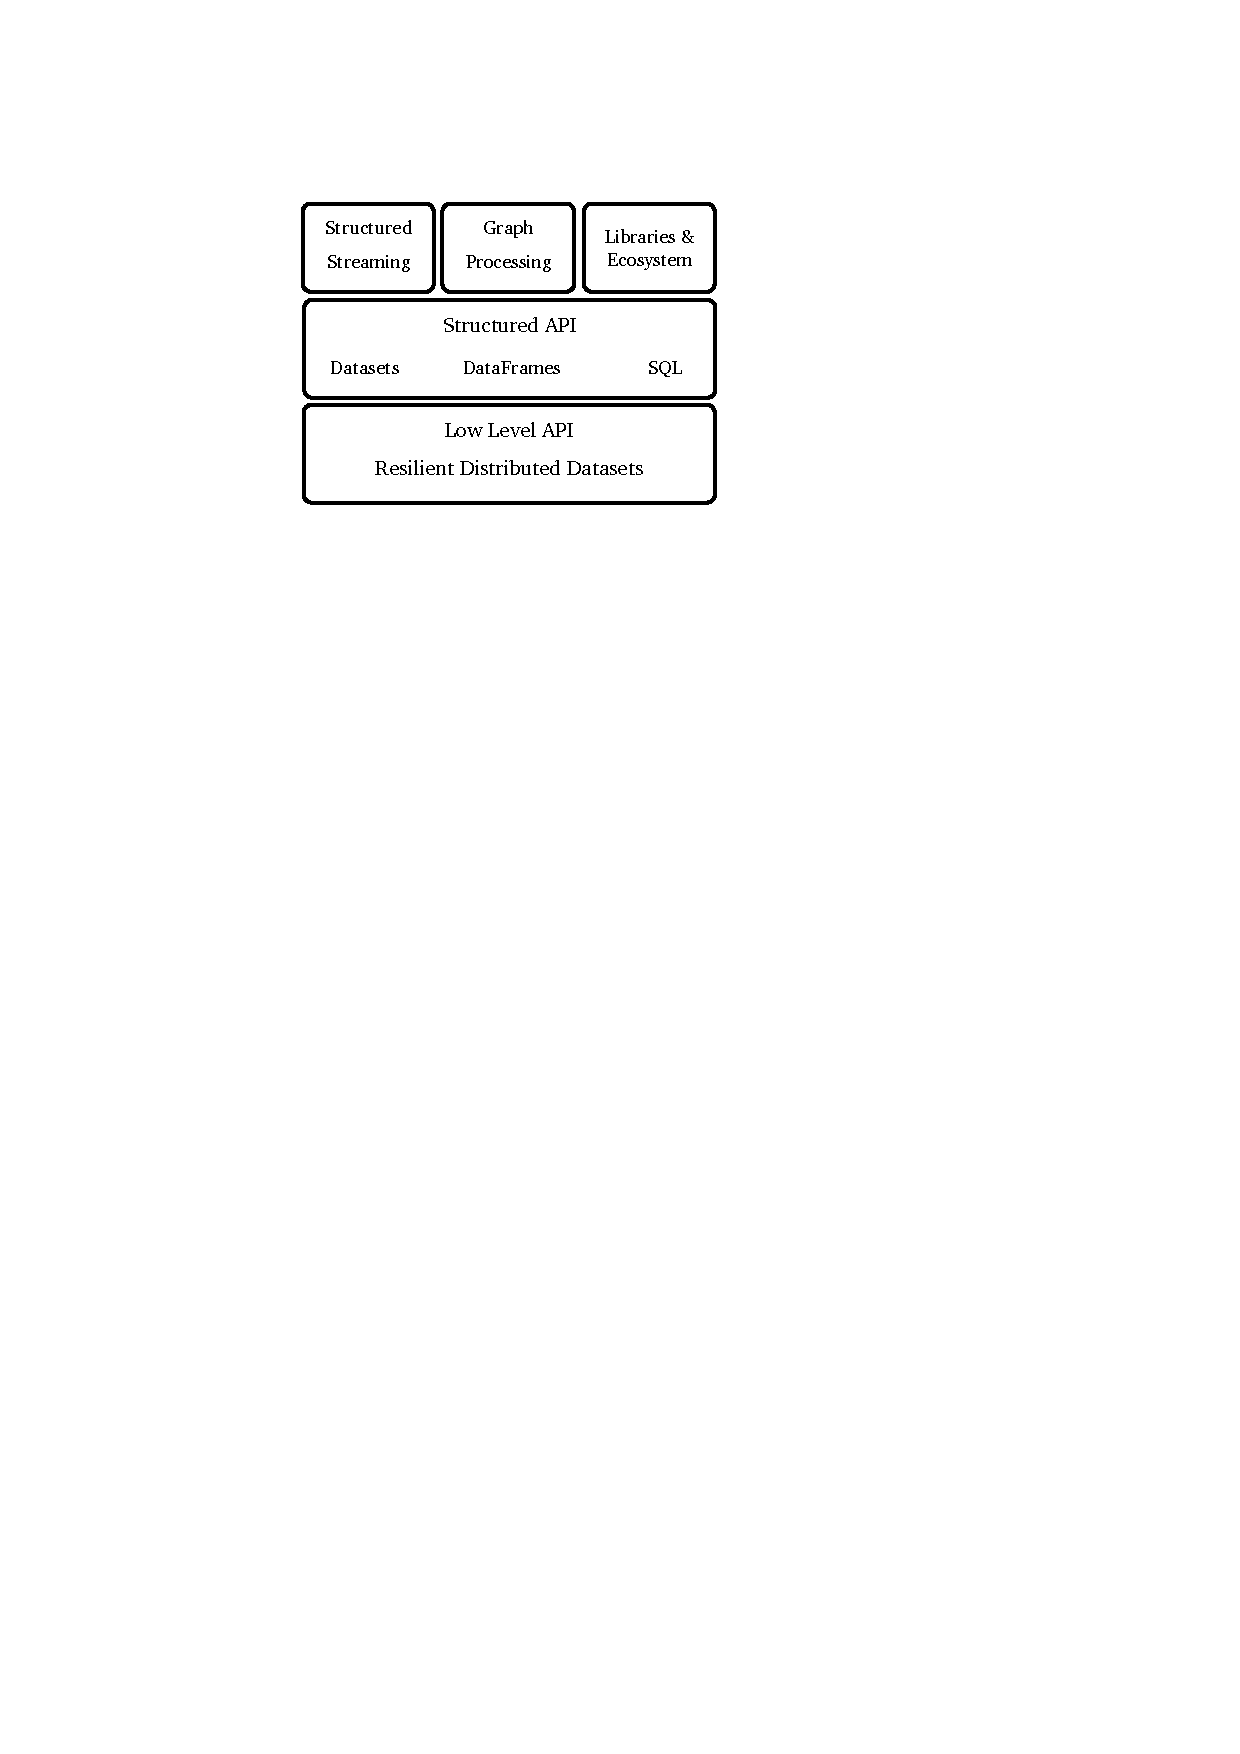
\includegraphics[clip,trim=5cm 21.2cm 8.7cm 3.4cm]{spark-eco.pdf}
    \caption{Apache Spark Stack}
    \label{fig:spark-eco}
\end{figure}

\subsection{Spark Application Architecture}
\label{sp:app}

\section{Resilient Distributed Datasets}
\label{sp:rdd}

\section{Discretized Streams}
\label{sp:dstream}

\section{Conclusion}
\label{sp:conc}

1. spark applications and executors. -->  graph here --> table for definitions
2. different modes of operation (mesos yarn standalone mode)
    1. mesos 
    2. yarn 
    3. standalone mode
    4. may be add graph
    5. add table for summerization

3. RDD

some examples on how RDD models 

DStreams

DStream paper

Spark Listener framework

